\documentclass[a4paper,12pt,french]{article}

\usepackage[utf8]{inputenc}
\usepackage[T1]{fontenc}
\usepackage{lmodern}
\usepackage{kpfonts}
\usepackage[margin=1.7cm]{geometry}
\usepackage{amsmath,amsfonts,amssymb}
\usepackage{enumitem}
\usepackage{tikz}
\usetikzlibrary{intersections}

\usepackage[np]{numprint}

\usepackage{babel}
\usepackage[]{exercise}

\setlist{noitemsep}
%\setlist[1]{\labelindent=\parindent} % < Usually a good idea
\setlist[itemize]{leftmargin=*}
\setlist[itemize,1]{label=$\triangleright$}
\setlist[enumerate]{labelsep=*, leftmargin=1.5pc}
\setlist[enumerate,1]{label=\arabic*., ref=\arabic*}
\setlist[enumerate,2]{label=\emph{\alph*}),
ref=\theenumi.\emph{\alph*}}
\setlist[enumerate,3]{label=\roman*), ref=\theenumii.\roman*}
\setlist[description]{font=\sffamily\bfseries}

\renewcommand{\ExerciseName}{Exercice}
\renewcommand{\AnswerName}{Réponse de l'exercice}
\renewcommand{\ExerciseHeader}{\textbf{\ExerciseName~\ExerciseHeaderNB}\hfill%
(\ExerciseTitle)\\[7mm]}

\newcommand{\N}{\mathbf{N}}
\renewcommand{\u}{(u_n)_{n\in\N}}

\everymath{\displaystyle\everymath{}}

\title{D.S. 1}
\date{7 octobre 2015}

\begin{document}

\maketitle

\begin{Exercise}[number=1,title={9 points}]
  Soit la suite numérique $\u$ définie sur $\N$ par : $u_0 =2$ et, pour
  tout entier naturel $n$, \[ u_{n+1} = \frac23 u_n + \frac13 n +1. \]
  \begin{enumerate}
    \item \begin{enumerate}
        \item Calculer $u_1$, $u_2$, $u_3$ et $u_4$. On pourra en donner
          des valeurs approchées à $10^{-2}$ près.
        \item Formuler une conjecture sur le sens de variation de cette
          suite.
      \end{enumerate}
    \item \begin{enumerate}
        \item Démontrer, par récurrence, que pour tout entier naturel
          $n,\ u_n \leqslant n+3$.
        \item Démontrer que pour tout entier naturel $n,\ u_{n+1} - u_n
          = \frac13\left(n+3 - u_n\right)$
        \item En déduire une validation de la conjecture précédente.
      \end{enumerate}
    \item On désigne par $(v_n)_{n\in\N}$ la suite définie sur $\N$ par
      $v_n = u_n -n$.
      \begin{enumerate}
        \item Démontrer  que la suite $(v_n)_{n\in\N}$ est une suite
          géométrique de raison $\frac23$.
        \item En déduire que pour tout entier naturel $n,\ u_n =
          2\times \left(\frac23\right)^n + n$.
        \item Déterminer la limite de la suite $\u$.
      \end{enumerate}
  \end{enumerate}
\end{Exercise}

\begin{Exercise}[number=2,title={5 points}]
  Dans un pays, il y a 2\% de la population contaminée par un virus. On
  dispose d'un test de dépistage de ce virus qui a les propriétés
  suivantes :
  \begin{itemize}[label=--]
    \item la probabilité qu'une personne contaminée ait un test positif
      est de \np{0.99} (sensibilité du test) ;
    \item la probabilité qu'une personne non contaminée ait un test
      négatif est de \np{0.97} (spécificité du test).
  \end{itemize}
  On fait passe un test à une personne choisie au hasard dans cette
  population. On note $V$ l'événement « la personne est contaminée par
  le virus », et  $T$ l'événement « le test est positif  ».

  \begin{enumerate}
    \item \begin{enumerate}
        \item Préciser les valeurs de probabilités $P(V)$, $P_V(T)$ et
          $P_{\overline{V}}(\overline{T})$.

          Construire un arbre de probabilité traduisant la situation.
        \item En déduire la probabilité de l'événement $V\cap T$.
      \end{enumerate}
    \item Démontrer que la probabilité que le test soit positif est de
      \np{0.0492}.
  \end{enumerate}
\end{Exercise}
\pagebreak
\begin{Exercise}[number=3,title={7 points}]
  Soit la suite numérique $(u_n)_{n\in\N}$ définie par $u_0 = 2$ et,
  pour tout entier naturel $n$ par \[ u_{n+1} = \frac15u_n + 3 \times
  \np{0.5}^n. \]
  \begin{enumerate}
    \item \begin{enumerate}
        \item Démontrer, par récurrence, que pour tout entier naturel
          non nul, on a : \[ u_n \geqslant \frac{15}4 \times
          \np{0.5}^n.\]
        \item En déduire, que pour tout entier naturel non nul, \[
          u_{n+1} - u_n \leqslant 0.\]
        \item Démontrer que la suite $(u_n)_{n\in\N}$ est convergente.
      \end{enumerate}
    \item On se propose dans cette question de déterminer la limite de
      la suite $(u_n)_{n\in\N}$.

      Soit $(v_n)_{n\in\N}$ la suite définie sur $\N$ par $v_n = u_n -
      10\times \np{0.5}^n$.
      \begin{enumerate}
        \item Démontrer que la suite $(v_n)_{n\in\N}$ est une suite
          géométrique de raison $\frac15$. On précisera le premier terme
          de la suite $(v_n)_{n\in\N}$.
        \item En déduire, que pour tout entier naturel, $u_n = -8 \times
          \left(\frac15\right)^n + 10\times \np{0.5}^n$.
        \item Déterminer la limite de la suite $(u_n)_{n\in\N}$.
      \end{enumerate}
  \end{enumerate}
\end{Exercise}
\vfill
\hfill \begin{quote}Personne ne nous chassera du paradis que Cantor a
créé pour nous.\end{quote}\hfill(David Hilbert)\vspace{2cm}
\pagebreak

\begin{Answer}[number=1]
  Soit la suite numérique $\u$ définie sur $\N$ par : $u_0 =2$ et, pour
  tout entier naturel $n$, \[ u_{n+1} = \frac23 u_n + \frac13 n +1. \]
  \begin{enumerate}
    \item \begin{enumerate}
        \item $u_1 = \frac43 + \frac13 + 1 = \frac83 \approx 2,67$, $u_2
          = \frac{16}9 + \frac23 + 1 = \frac{31}9i \approx 3,44$, $u_3 =
          \frac{116}{27} \approx 4,30$ et $u_4 = \frac{421}{81} \approx
          5,20$.
        \item La suite semble être croissante non majorée, et diverger
          vers $+\infty$.
      \end{enumerate}
    \item \begin{enumerate}
        \item \begin{itemize}
            \item $n=0\ :\ u_0 = 2 \leqslant 0 + 3 = 0$ est vraie.
            \item $u_n \leqslant n+3 \implies \frac23 u_n \leqslant
              \frac23 n + 2 \implies \frac23 u_n + \frac13 n \leqslant
              n + 2 \implies u_{n+1} \leqslant n + 1 + 3$
            \item $P_O$ vraie et pour $n$ fixé, $P_n \implies P_{n+1}$
              font que la propriété est vraie pour tout $n\in\N$.
            \item Soit $n$ fixé, $u_{n+1} - u_n = \frac13 (n + 3) -
              \frac13n = \frac13\left(n+3 - u_n\right)$
          \end{itemize}
        \item La dernière égalité et l'inégalité précédente permettent
          d'écrire que $\forall n\in\N,\ u_{n+1} - u_n \geqslant 0$, ce
          qui valide que la suite est strictement croissante.
      \end{enumerate}
    \item On désigne par $(v_n)_{n\in\N}$ la suite définie sur $\N$ par
      $v_n = u_n -n$.
      \begin{enumerate}
        \item $\dfrac{v_{n+1}}{v_n} = \dfrac{\frac23u_n - \frac23n}{u_n
          - n}=\frac23$
        \item $v_0 = 2 \ v_n =2\left(\frac23\right)^n \ u_n = 2\times
          \left(\frac23\right)^n + n$.
        \item $\lim_{n\to+\infty}u_n = +\infty$.
      \end{enumerate}
  \end{enumerate}
\end{Answer}

\begin{Answer}[number=2]
  Dans un pays, il y a 2\% de la population contaminée par un virus. On
  dispose d'un test de dépistage de ce virus qui a les propriétés
  suivantes :
  \begin{itemize}[label=--]
    \item la probabilité qu'une personne contaminée ait un test positif
      est de \np{0.99} (sensibilité du test) ;
    \item la probabilité qu'une personne non contaminée ait un test
      négatif est de \np{0.97} (spécificité du test).
  \end{itemize}
  On fait passe un test à une personne choisie au hasard dans cette
  population. On note $V$ l'événement « la personne est contaminée par
  le virus », et  $T$ l'événement « le test est positif  ».

  \begin{enumerate}
    \item \begin{enumerate}
        \item $P(V) = 0,02$, $P_V(T) = 0,99$ et
          $P_{\overline{V}}(\overline{T}) = 0.97$.

          \begin{center}
            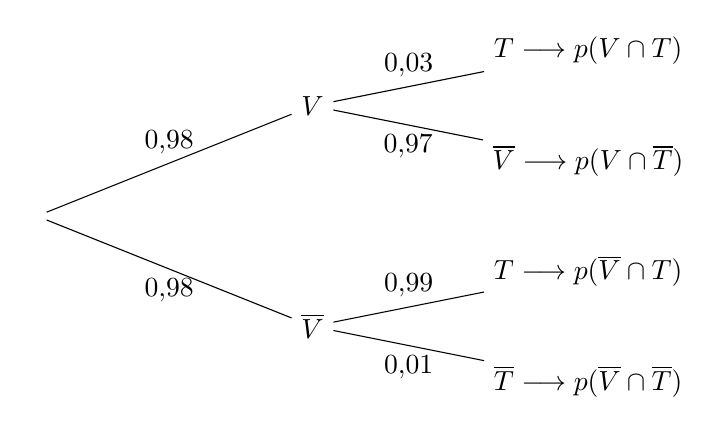
\begin{tikzpicture}[scale=1.4,level distance=25mm,sibling distance=10mm]
              \node {} [grow=right]
              child[sibling distance=20mm] {
                node {$\overline{V}$}
                child[sibling distance=10mm] {
                  node {$\overline{T} \longrightarrow p(\overline{V}
                  \cap\overline{T})$}
                  edge from parent node[below] {$\np{0.01}$}
                }
                child[sibling distance=10mm] {
                  node {$T \longrightarrow p(\overline{V} \cap T)$}
                  edge from parent node[above] {$\np{0.99}$}
                }
                edge from parent node[below] { $\np{0.98}$ }
              }
              child[sibling distance=20mm] { node {$V$}
                child[sibling distance=10mm] {
                  node {$\overline{V} \longrightarrow p(V\cap\overline{T})$}
                  edge from parent node[below] { $\np{0.97}$ }
                }
                child[sibling distance=10mm] {
                  node {$T \longrightarrow p(V\cap T)$}
                  edge from parent node[above] { $\np{0.03}$ }
                }
                edge from parent node[above] { $\np{0.98}$ }
              } ;
            \end{tikzpicture}
          \end{center}
        \item $p(V\cap T) = \np{0.0198}$.
      \end{enumerate}
    \item $p(T) = p(V\cap T) + p(overline{V} \cap T) = \np{0.0198} +
      \np{0.0294} = \np{0.0492}.$
  \end{enumerate}
\end{Answer}

\begin{Answer}[number=3]
  \begin{enumerate}
    \item \begin{enumerate}
        \item \begin{itemize}
            \item $u_1 = \frac25 +3 = \frac{17}5 \geqslant
              \frac{15}4\times \np{0.5} = \frac{15}{8}$ ($u_1 \geqslant
              3$ et $\frac{15}8 \leqslant 2$)
            \item $u_n \geqslant \frac{15}4 \times \np{0.5}^n \implies
              \frac15 u_n \geqslant \frac34 \times \np{0.5}^n \implies
              u_{n+1} \geqslant \frac34 \times \np{0.5}^n + 3 \times
              \np{0.5}^n = \frac{15}4 \times \np{0.5}^n \geqslant
              \frac{15}4 \times \np{0.5}^{n+1}$
          \end{itemize}
        \item $u_{n+1} - u_n = \frac{-4}5u_n + 3 \times \np{0.5}^n
          \geqslant \frac{-4}5\times \frac{15}4 \times \np{0.5}^n + 3
          \times \np{0.5}^n = 0$
        \item $u_n$ décroissante minorée, donc convergente.
      \end{enumerate}
    \item \begin{enumerate}
        \item $v_n = u_n - 10\times \np{0.5}^n \implies v_0 = -8$.

          $v_n+1 = u_{n+1} - 10 \times \np{0.5}^{n+1} = \frac15 u_n + 3
          \times \np{0.5}^n - 5 \times \np{0.5}^n = \frac15 u_n -2
          \times \np{0.5}^n = \frac15 v_n$

        \item $v_n = -8\left(\frac15\right)^n$

          $u_n = v_n + 10\times \np{0.5}^n = -8\left(\frac15\right)^n
          +10\times \np{0.5}^n$

        \item $\lim_{n\to+\infty} u_n = 0$
      \end{enumerate}
  \end{enumerate}
\end{Answer}

\end{document}
